\begin{figure}[htbp]
\centering
\begin{tikzpicture}[x=1cm,y=1cm]
\node[anchor=south west,inner sep=0] at (0,0) {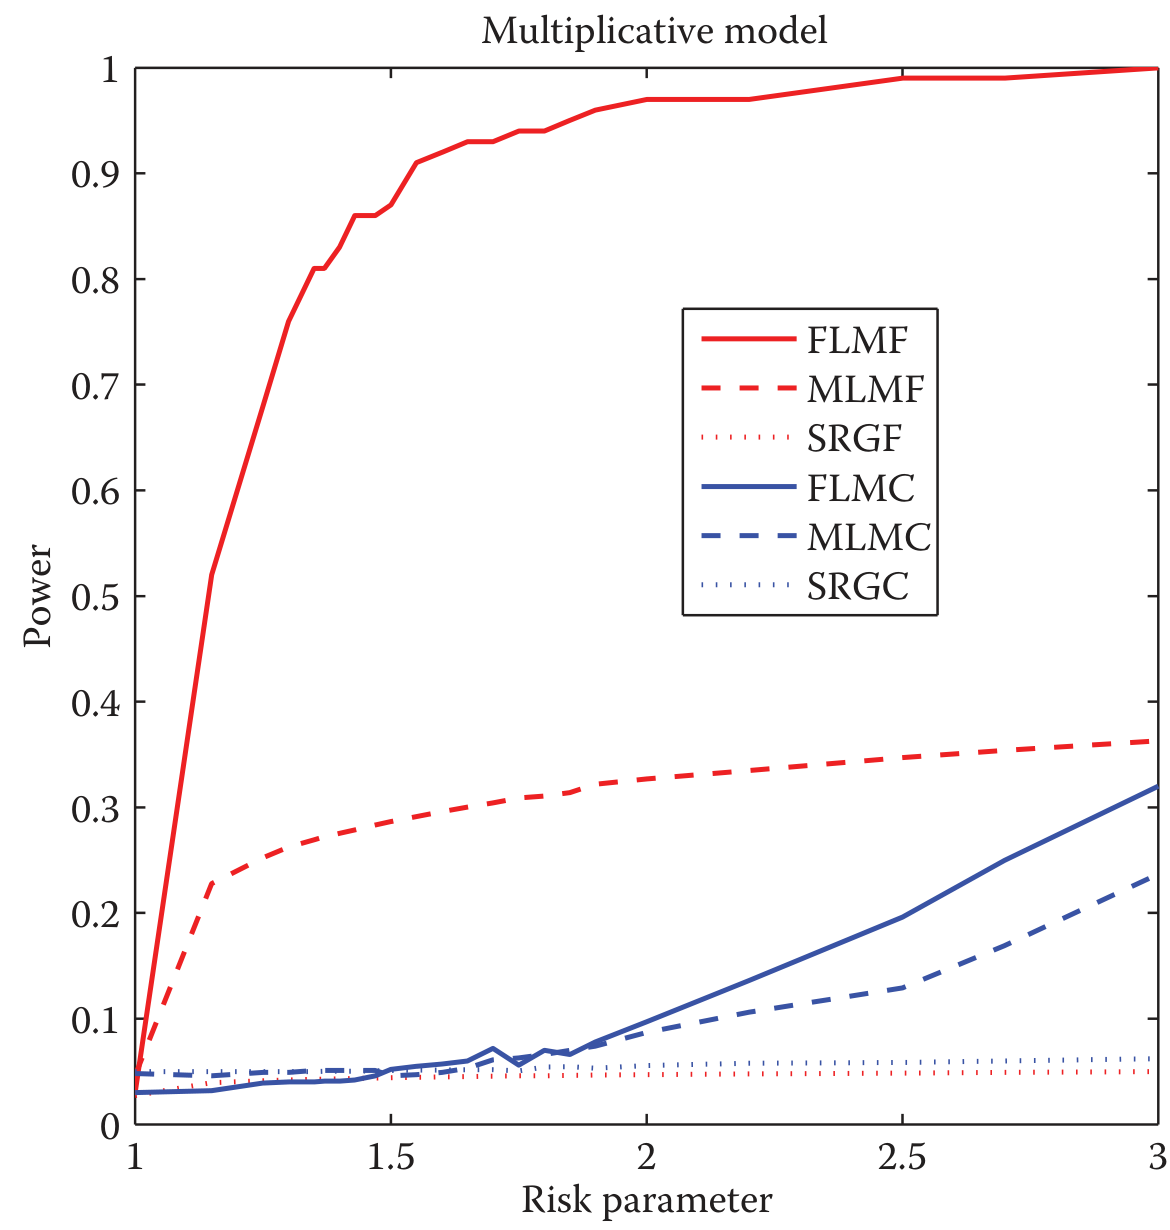
\includegraphics[width=13.0cm]{figures/ch03_fig17_data.png}};
\fill[white] (5.7575,0.0651) rectangle (8.6264,0.5651);
\node[font=\small,rotate=0,inner sep=0] at (7.1919,0.3151) {风险参数};
\fill[white] (0.1867,6.4263) rectangle (0.6978,7.6543);
\node[font=\small,rotate=90,inner sep=0] at (0.4423,7.0403) {统计功效};
\fill[white] (5.3085,13.0487) rectangle (9.2352,13.5487);
\node[font=\small,rotate=0,inner sep=0] at (7.2718,13.2987) {乘性模型};
\end{tikzpicture}
\origfig{17}{乘性模型下，六种模型的统计功效随风险参数的变化曲线。}
\label{fig:ch03-17}
\end{figure}
